\chapter{Introducción}

\subsection{Regiones activas.}
Las regiones activas son zonas en el Sol comparables con el tamaño de la tierra con una fuerte presencia de campo magnético, es decir, un área donde las lineas de campo internas del Sol pueden emerger de la fotósfera creando un bucle con polaridad negativa de un lado y positiva del otro, este particular fenómeno hace que se arrastre plasma de la superficie a zonas más altas en la atmósfera solar causando un cambio de densidad y enfriando el plasma; esto hace que en observaciones en el visible las manchas solares se vean oscuras, dado que su temperatura es levemente menor (4000K) a la de la fotósfera  (5777K).\\
Estas regiones debido a que concentran una gran intensidad de campo magnético confinado son epicentro de eventos muy energéticos como lo son las \textbf{erupciones solares} que ocurren en la cromosfera y las \textbf{eyecciones de masa coronal (CME)} en la corona solar. Estos eventos se generan cuando la concentración de campo es tan fuerte que se genera el fenómeno llamado \textbf{reconexión magnética} en el cual las lineas de campo se cruzan, generando una explosión que arrastra todo el plasma confinado en el bucle, dependiendo de que tan energético sea esta, podrá arrojar material hasta ser desprendido del Sol como es el caso de las CME.\\

Puesto que no se pueden predecir esta clase de eventos, actualmente se estudian con ayuda de satélites y observaciones terrestres en gran parte del espectro electro magnético e incluso en altas energías como los rayos X debido a la fuerte aceleración que pueden sufrir los iones al interior del bucle.



%%%%%%%%%%%--------------------------------------%%%%%%%%%%%%%%%%%%%%%%---------------%%%%%%%%%%%%%%%%%%%%%%%%%%

\subsection{Fibras ópticas.}
Las fibras ópticas son un elemento óptico el cual se basa en un caso especial que experimenta la luz sobre una interfaz que divide dos medios con diferente permitividad eléctrica y permeabilidad magnética llamado \textbf{reflexión total}, dicha reflexión también depende del ángulo entre el frente de onda de la fuente y el vector normal a la interfaz, de esta manera la fibra óptica se comporta como una guía de onda para IR-VIS-UV.\\
Para hacer una mejor descripción del fenómeno suponemos polarización paralela con lo cual se desarrollarán las ecuaciones de continuidad que deben cumplir los campos incidente, reflejado y transmitido al interactuar con la interfaz entre los dos medios, dichas ecuaciones dan resultado a la \textbf{ley de Snell} y a las \textbf{ecuaciones de Fresnel}. 

\begin{figure}[H]
\centering
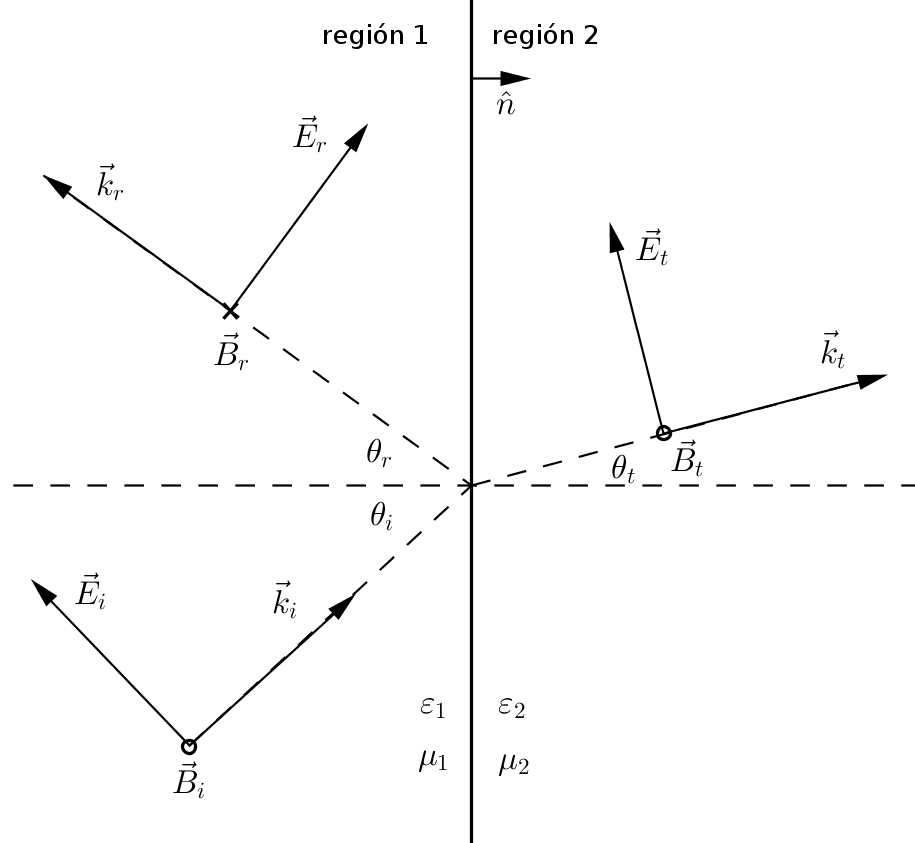
\includegraphics[width=0.46\linewidth]{Kap1/interfaz.png}
\caption{Incidencia oblicua de una onda plana, caso polarización paralela para dos medios con $\varepsilon_1$,$\mu_1$ y $\varepsilon_2$,$\mu_2$ respectivamente.} 
\label{interfaz}
\end{figure}

En la figura \ref{interfaz} se muestra la signatura y orientación escogida para los campos eléctrico y magnético antes y después de interactuar con la interfaz, ya con esto podemos obtener la ley de Snell a partir de la continuidad en las componentes tangenciales, de los campos incluido el vector de onda, es decir las componentes paralelas a la superficie de interfase así como la componente paralela del vector de onda. Esto lo podemos escribir como

\begin{equation}\label{continuidad}
    \hat{n} \times (\Vec{E}_2 - \Vec{E}_1) = 0 \hspace{3mm}\text{ y }\hspace{3mm}\hat{n} \times (\Vec{H}_2 - \Vec{H}_1) = 0
\end{equation}
con lo cual usando (\ref{continuidad}) se obtiene
\begin{equation}\label{continuidad2}
    k_{i,\parallel} = k_{r,\parallel} = k_{t,\parallel} = k_{\parallel} \xrightarrow{} k_{\parallel}=k_i \sin{\theta_i}=k_r \sin{\theta_r}=k_t \sin{\theta_t}.
\end{equation}
Usando la relación de dispersión para cada medio $k=\frac{\omega}{v}=\frac{\omega}{c}\frac{c}{v}=\frac{\omega}{v}n$ donde $n$,$v$ son el índice de refracción y velocidad de la onda en el medio respectivamente, resultando:
\begin{equation}\label{snell}
    n_i\sin{\theta_i}=n_r\sin{\theta_r}=n_t\sin{\theta_t}=cte \hspace{15mm}\text{\textbf{Ley de Snell.}}
\end{equation}
Ahora usando la ecuación (\ref{snell}) imponemos una condición para que el haz sea transmitido al límite de $\theta_t=\pi/2$ despejando tenemos
\begin{equation}\label{total}
    \theta_c = \arcsin{\frac{n_2}{n_1}}
\end{equation}
donde $\theta_c$ es el ángulo mínimo de incidencia con $n_2<n_1$, dicha condición es la que da lugar a la \textbf{reflexión total interna} dado que todo haz que incida con un ángulo mayor tendrá componente netamente reflejada; a éste ángulo lo denominamos \textbf{ángulo crítico}.

\begin{figure}[H]
\centering
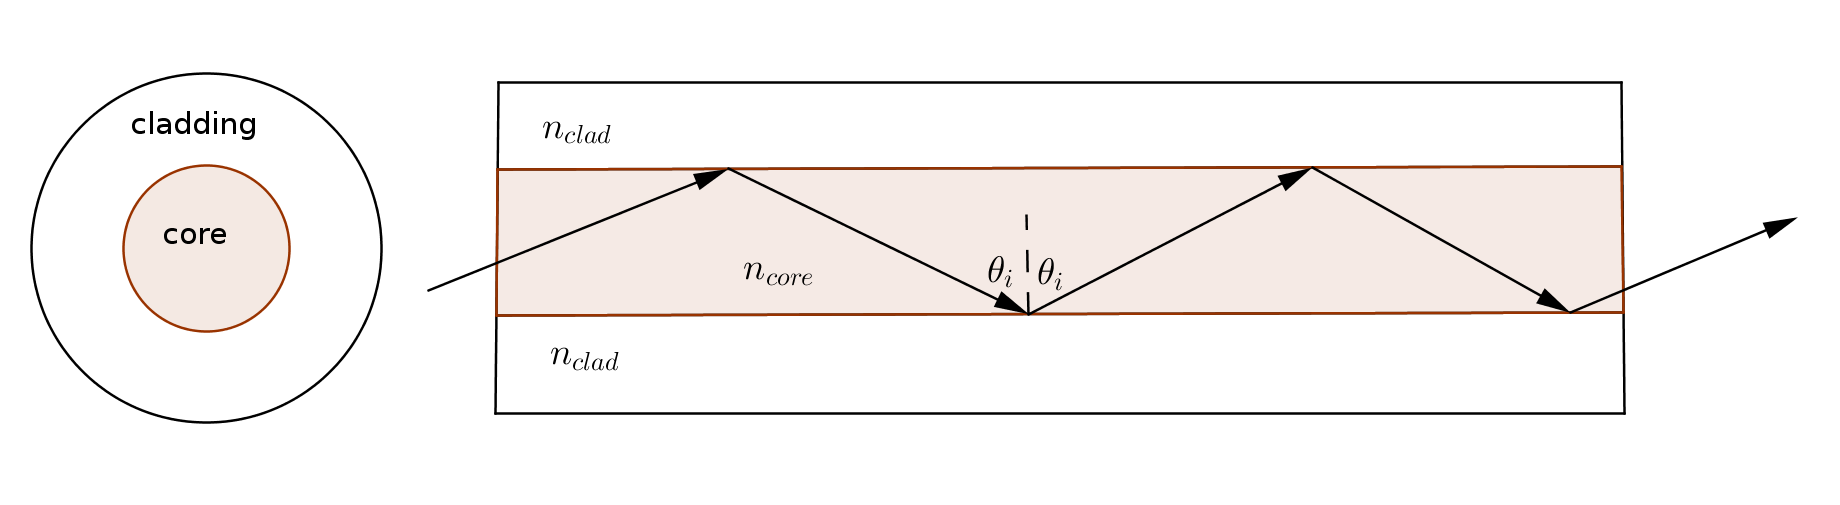
\includegraphics[width=0.76\linewidth]{Kap1/fibra.png}
\caption{Comportamiento de un haz al interior de una fibra óptica.} 
\label{fibra}
\end{figure}
En la figura \ref{fibra} se muestra el esquema de una fibra óptica la cual se compone de dos regiones con diferentes índices de refracción llamados núcleo (core) y revestimiento (cladding) donde $n_{clad}<n_{core}$, así todo haz que cumpla la relación (\ref{total}) se propagará dentro del núcleo, mientras que para ángulos menores los haces serán absorbidos por el revestimiento.


%%%%----------------------------------------------%%%%
%%%%----------------------------------------------%%%%

\subsection{Propiedades ópticas de las fibras.}
Ya entendido el mecanismo de trasporte en una fibra óptica entraremos más en detalle a propiedades importantes de éste elemento óptico como lo son la atenuación de la señal y optimización para diferentes longitudes de onda los cuales dependen en gran parte de los procesos de construcción.\\
Puesto que las propiedades suelen cambiar dependiendo del tipo de construcción se explicarán los tipos de fibras más usuales.

\begin{figure}[H]
\centering
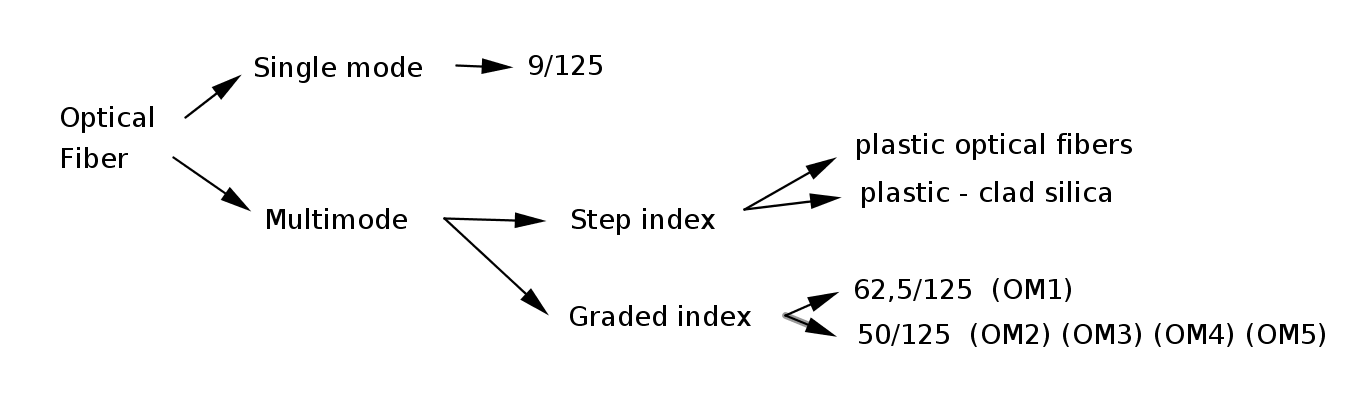
\includegraphics[width=0.76\linewidth]{Kap1/tipos_fibras.png}
\caption{Tipos de fibras ópticas más comunes en el mercado donde se muestran los tamaños de fibras más usados; diámetro núcleo/diámetro revestimiento en $\mu$m.} 
\label{tipos_fibras}
\end{figure}

En la figura \ref{tipos_fibras} se observan las fibras ópticas comúnmente usadas dentro de las cuales resaltan tres grandes grupos, las fibras monomodo , multimodo con salto de índice y multimodo con gradiente de índice. Las fibras monomodo se destacan precisamente por privilegiar un único camino en el cual se propaga la onda, con lo cual se reducen efectos de dispersión cromática y \textbf{dispersión modal} la cual se produce por un retraso temporal en la propagación de los haces de luz debida a los múltiples caminos ópticos que puede tomar para una misma longitud de onda; dichas fibras suelen tener fuentes LASER de alta potencia alrededor de los 1300-1550 nm con lo cual consiguen transmitir una alta taza de información a distancias hasta de 400 Km.

\begin{figure}[H]
\centering
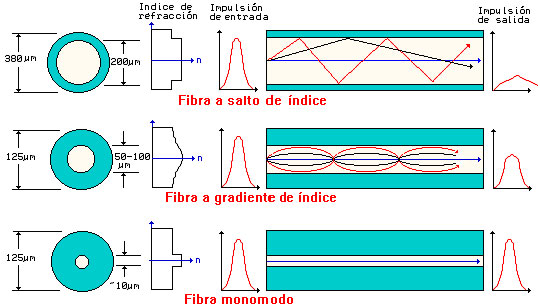
\includegraphics[width=0.66\linewidth]{Kap1/fibras3.jpg}
\caption{Tipos de fabricación tanto en escala-tamaño como en variación de índice de refracción en función del radio. Tomado de \textit{https://es.wikipedia.org/wiki/Fibra-optica}} 
\label{fibras3}
\end{figure} 
%sacada de: referencia

Por otro lado las fibras multimodo al tener un núcleo más grande permiten al haz de luz recorrer distintos caminos ópticos lo cual introduce dispersión modal, por esto existen dos tipos de fibras multimodo como se muestra en la figura \ref{fibras3}, las fibras de índice escalonado se compone de dos únicos materiales lo cual aumenta la dispersión modal y cromática (dichas fibras dadas sus limitaciones pero fácil construcción son usadas para enlaces cortos 100m). Ahora las fibras con gradiente de índice se construyen a partir de pequeños saltos de índice siguiendo una distribución parabólica de manera discreta puesto que por cuestiones de fabricación no es posible variar el índice de manera continua, dicha disposición contribuye a la reducción de la dispersión modal y dispersión cromática en función de la longitud de onda de la fuente aumentando el alcance al orden de 2km. Puesto que las fibras multimodo son para enlaces cortos tienden a tener un mayor rango de tolerancia en cuanto a fuentes con lo cual suelen venir optimizadas entre 800-1300 nm.\\

Puesto que los procesos de fabricación no son perfectos pueden presentarse perdidas de intensidad de la onda por dispersión o absorción propia del material, dentro de la dispersión se tienen varias contribuciones como ya se ha mencionado la dispersión cromática y modal, pero además se cuenta con un Scattering o dispersión de Rayleigh el cual se produce por la interacción de la luz con microscópicas irregularidades o estrés en el material producidas durante la fabricación del mismo, esto hace que la luz se disperse en otras direcciones incluso superando el ángulo critico siendo absorbida en el revestimiento.
Por ultimo tenemos la absorción la cual se da cuando la luz interactúa con átomos en el material usados para dopar y cambiar el índice de refracción al ser absorbido el fotón puede ser que el fotón emitido salga en otra dirección y se salga del núcleo terminando siendo absorbido en el revestimiento.

\begin{figure}[H]
\centering
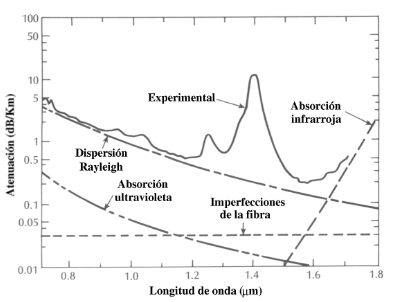
\includegraphics[width=0.56\linewidth]{Kap1/atenuacion.png}
\caption{Contribuciones en la atenuación de la onda en una fibra óptica en función de la longitud de onda de la fuente. Tomado de \textit{http://www.iuma.ulpgc.es/users/jrsendra/Docencia}.} 
\label{atenuacion}
\end{figure} 

En la figura \ref{atenuacion} se observan los efectos que producen atenuación de la señal en función de la longitud de onda según la región de operación de la fibra óptica. En el caso de la absorción suelen haber picos con la interacción de moléculas $OH+$ los cuales comúnmente se encuentran en los 1000, 1400 y 1600 nm creando ventanas en donde es óptima la transmisión, en éstas ventanas suelen trabajar las fibras monomodo y algunas multimodo de gradiente de índice.

%%%%----------------------------------------------%%%%
%%%%----------------------------------------------%%%%

\subsection{Teoría de difracción para las aberturas rectangular y circular.}

En esta sección se explicará la teoría básica de la abertura rectangular \textit{Slit} en inglés, y la abertura circular, los cuales son elementos ópticos importantes en el funcionamiento de cualquier espectrógrafo convencional. La teoría que presentamos acá está basada en la aproximación de Fraunhofer, es decir, el ancho de la abertura es mucho menor a la distancia entre el plano que contiene la abertura y el plano donde mediremos el patrón de difracción producido, esto es

\begin{equation}\label{aprox_fran}
    N=\left[ \frac{{(x+y)}^2}{2d}\right]\frac{2}{\lambda}\ll 1,
\end{equation}
donde $N$ es el número de zonas de Fresnel, &(x,y)& describen la abertura y $d$ la distancia entre los planos.\\

Para calcular el patrón de difracción producido por los orificios usaremos la integral de difracción de Fraunhofer, la cual es una aproximación generada de la integral de difracción de Fresnel aplicando la ecuacion (\ref{aprox_fran}), esto puede ser visto como el número de zonas de Fresnel que caben en la apertura con $N\ll 1$, dicha expresión está escrita de la siguiente manera:

\begin{equation}\label{difraccion_fraunhofer}
    I(x',y')=I(u\lambda d,v\lambda d)=\frac{1}{\lambda^2 d^2}|\mathcal{F}\lbrace E(x,y) \rbrace |^2 ,
\end{equation}
en la cual las variables primadas $(x',y')$ se ubican en un plano paralelo separado una distancia $d$ al plano donde se encuentra la abertura con variables $(x,y)$, dicho esto veamos como se procede a calcular la irradiancia para las aberturas de interés.

\begin{itemize}
    \item \textbf{Rendija rectangular.}\\
    Dada la simetría para la abertura rectangular, haremos de coordenadas cartesianas para expresar el campo eléctrico en el plano de la abertura, haciendo uso de la función rectángulo $rect(x)$ tenemos,
    \begin{equation}\label{campo_rect}
        E(x,y)=E_0 \hspace{2mm} rect(x/a) \hspace{2mm} rect(y/b)\hspace{5mm}\text{ donde }\hspace{5mm}rect(x/a) = \left\lbrace
        \begin{array}{ll}
            \textup{si } |x|\leq a/2 & 1\\
            \textup{si } |x| > a/2 & 0
        \end{array}
        \right.
    \end{equation}
    
        \begin{figure}[H]
    \centering
    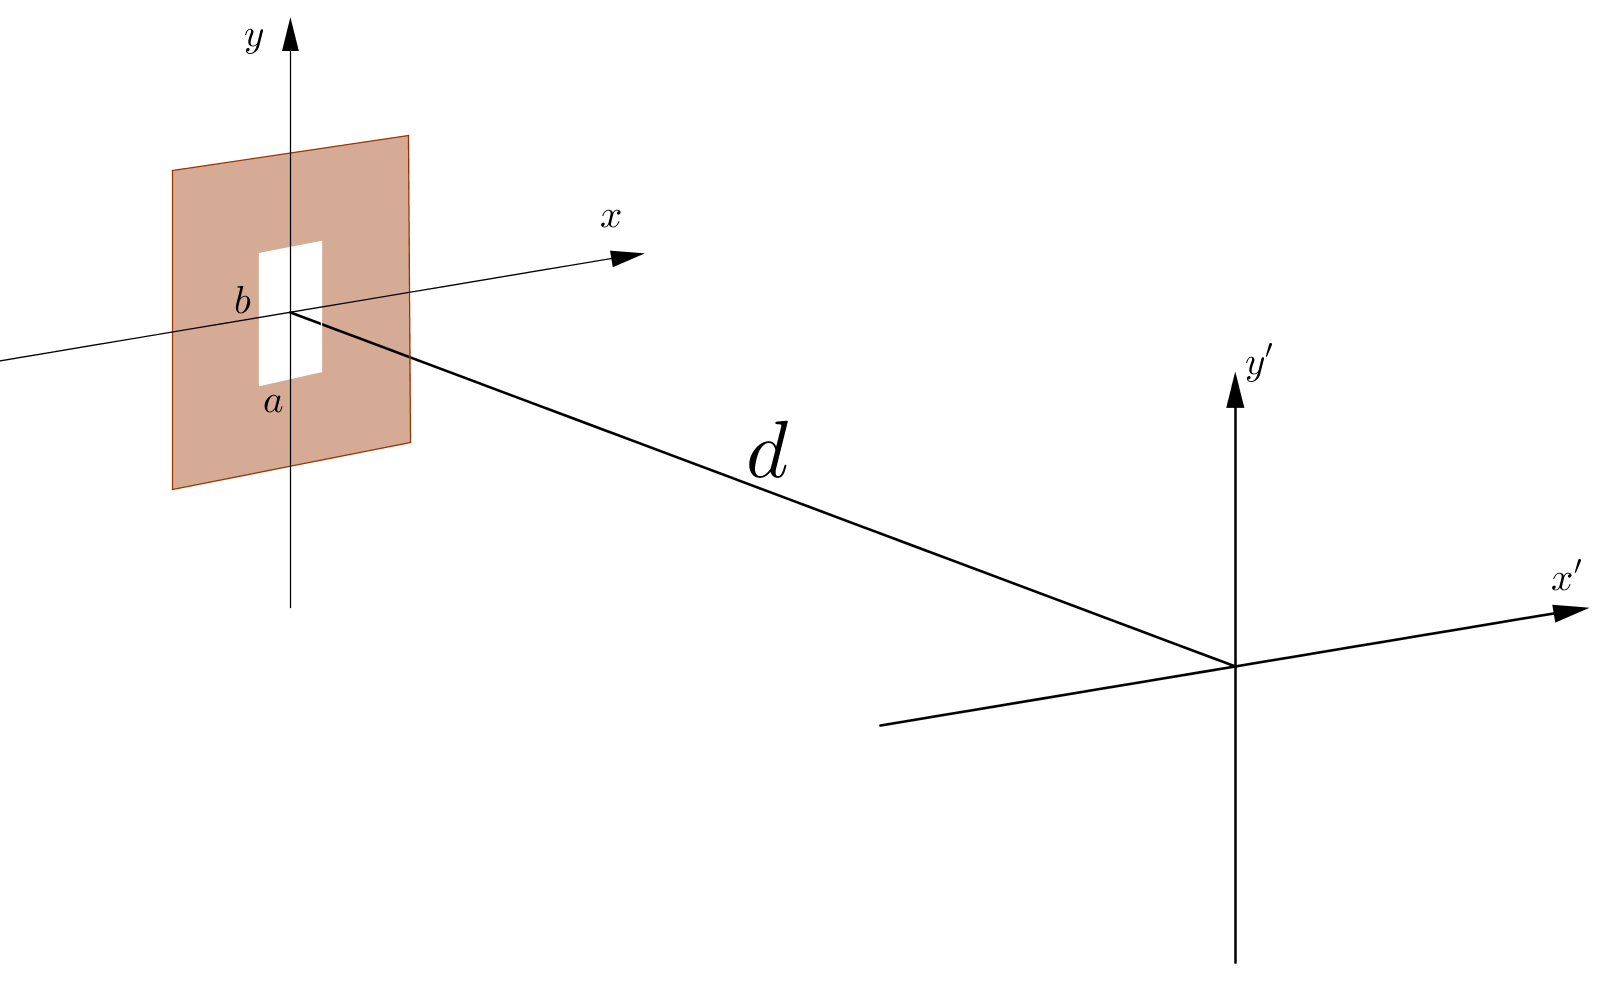
\includegraphics[width=0.75\linewidth]{Kap1/apertura_rect.png}
    \caption{Esquema  apertura rectangular aproximación de Fraunhofer.} 
    \label{abertura_rect}
    \end{figure}
    
    En la figura \ref{abertura_rect} se muestra la situación planteada, con lo cual una vez expresado el campo $E$ procedemos a hallar la irradiancia $I$ usando la ecuación (\ref{campo_rect}) en (\ref{difraccion_fraunhofer}) de la siguiente manera
    
    \begin{eqnarray}
        I(x',y')&=&\frac{1}{\lambda^2 d^2} \left |\int_{-\infty}^{\infty} \int_{-\infty}^{\infty} E(x,y) e^{-2\pi i (ux+vy)}dx dy \right |^2\\
        &=&\frac{1}{\lambda^2 d^2} \left |\int_{-a/2}^{a/2} \int_{-b/2}^{b/2} E_0 e^{-2\pi i (ux+vy)}dx dy \right |^2\\
        &=&\frac{E_0}{\lambda^2 d^2} \left |\int_{-a/2}^{a/2} e^{-2\pi i ux} dx\int_{-b/2}^{b/2} e^{-2\pi i vy} dy \right |^2,
    \end{eqnarray}
    
    calculando la integral en $x$ (de manera similar para $y$) 
    
    \begin{eqnarray}
        \int_{-a/2}^{a/2} e^{-2\pi i ux} dx &=&\left\frac{-1}{2\pi i u}  e^{-2\pi i ux}\right |_{-a/2}^{a/2} = \frac{-i}{2\pi u}\left[ -e^{-\pi i ua} + e^{\pi i ua}\right] \\ 
         &=&\frac{-i(2i)}{2\pi u}\sin{(\pi u a)}\frac{a}{a} = a \hspace{1mm} sinc(\pi x'a/\lambda d),
    \end{eqnarray}

    con lo cual finalmente se obtiene la expresión 
    
    \begin{equation}
        I(x',y')=I_0 \hspace{1mm}{sinc}^2\left(\frac{\pi x' a}{\lambda d} \right) \hspace{1mm}{sinc}^2\left(\frac{\pi y' b}{\lambda d} \right)\hspace{4mm}\text{ con }\hspace{4mm} I_0=\frac{E_0^2 a^2 b^2}{\lambda^2 d^2}
    \end{equation}
    
    \begin{figure}[H]
    \centering
    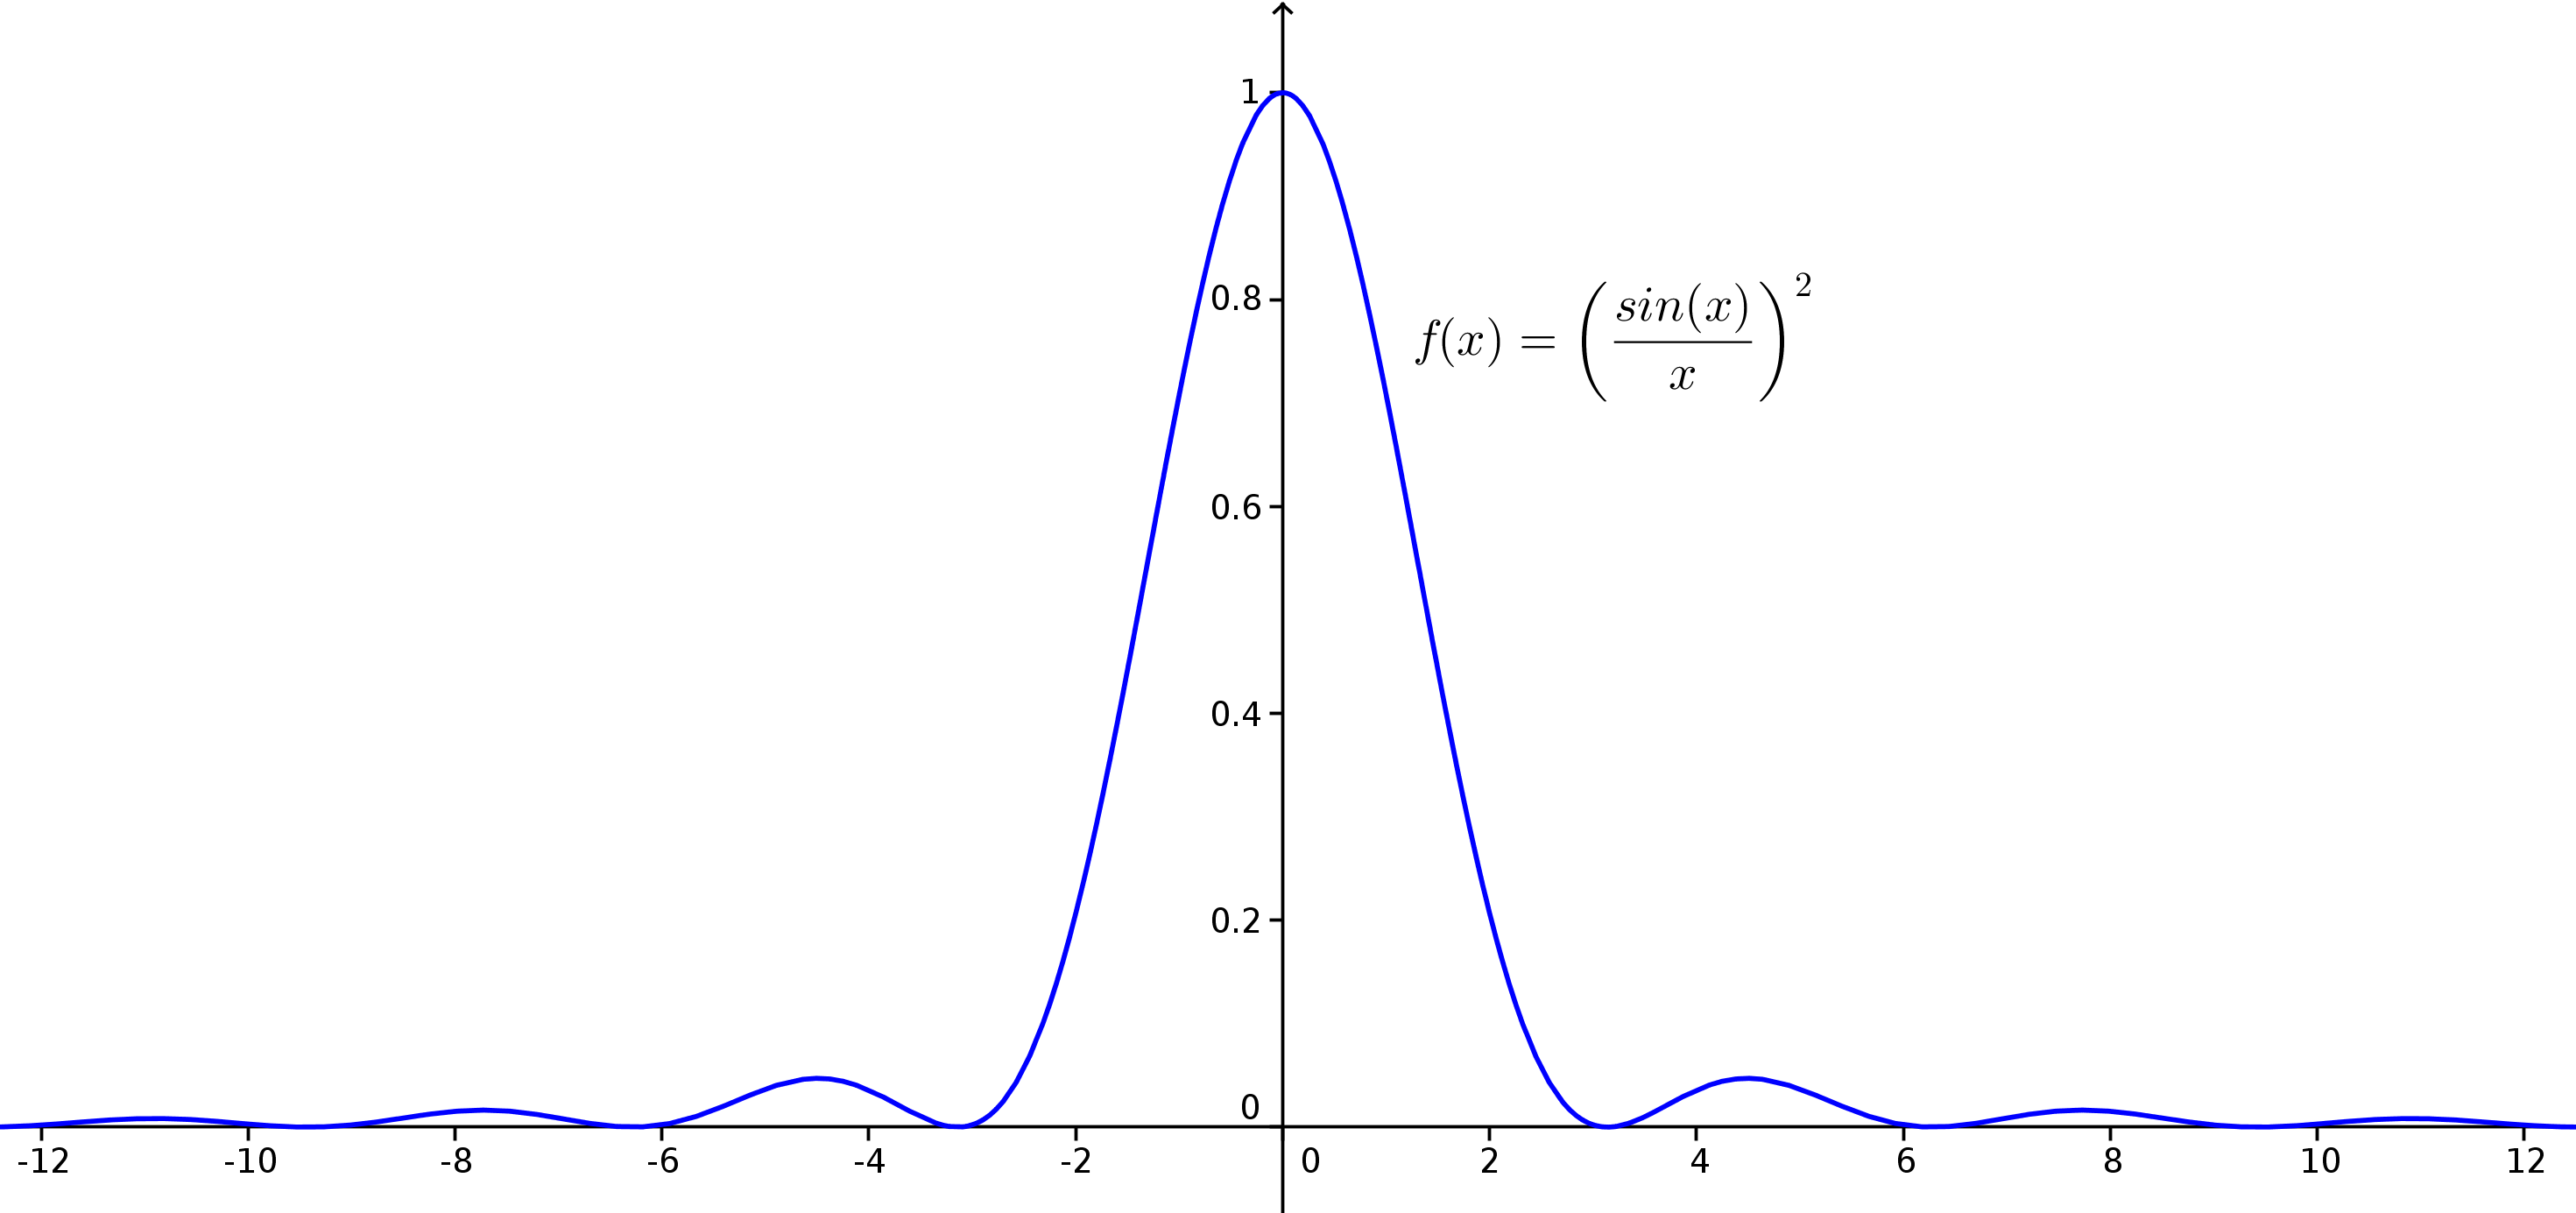
\includegraphics[width=0.75\linewidth]{Kap1/sinc.png}
    \caption{Gráfica de la función ${sinc}^2(x)$.} 
    \label{sinc}
    \end{figure}
    
    la ecuación (\ref{irrad_rect}) nos muestra el patrón de difracción generado por la abertura, donde se observan máximos y mínimos de radiación modulados por una función seno en cada eje. Como ejemplo se tiene al \textbf{Slit} el cual puede tener el orden de pocos centímetros de alto y un orden de micras de ancho, es decir, se observa con mayor claridad un patrón en una dirección que en otra. la figura \ref{sinc} describe el comportamiento de la función ${sinc}^2(x)$ la cual tiene un máximo de irradiancia en el origen y se puede ver como un patrón unidimensional similar al Slit.
    
    \item \textbf{Apertura circular.}\\
    
    \begin{figure}[H]
    \centering
    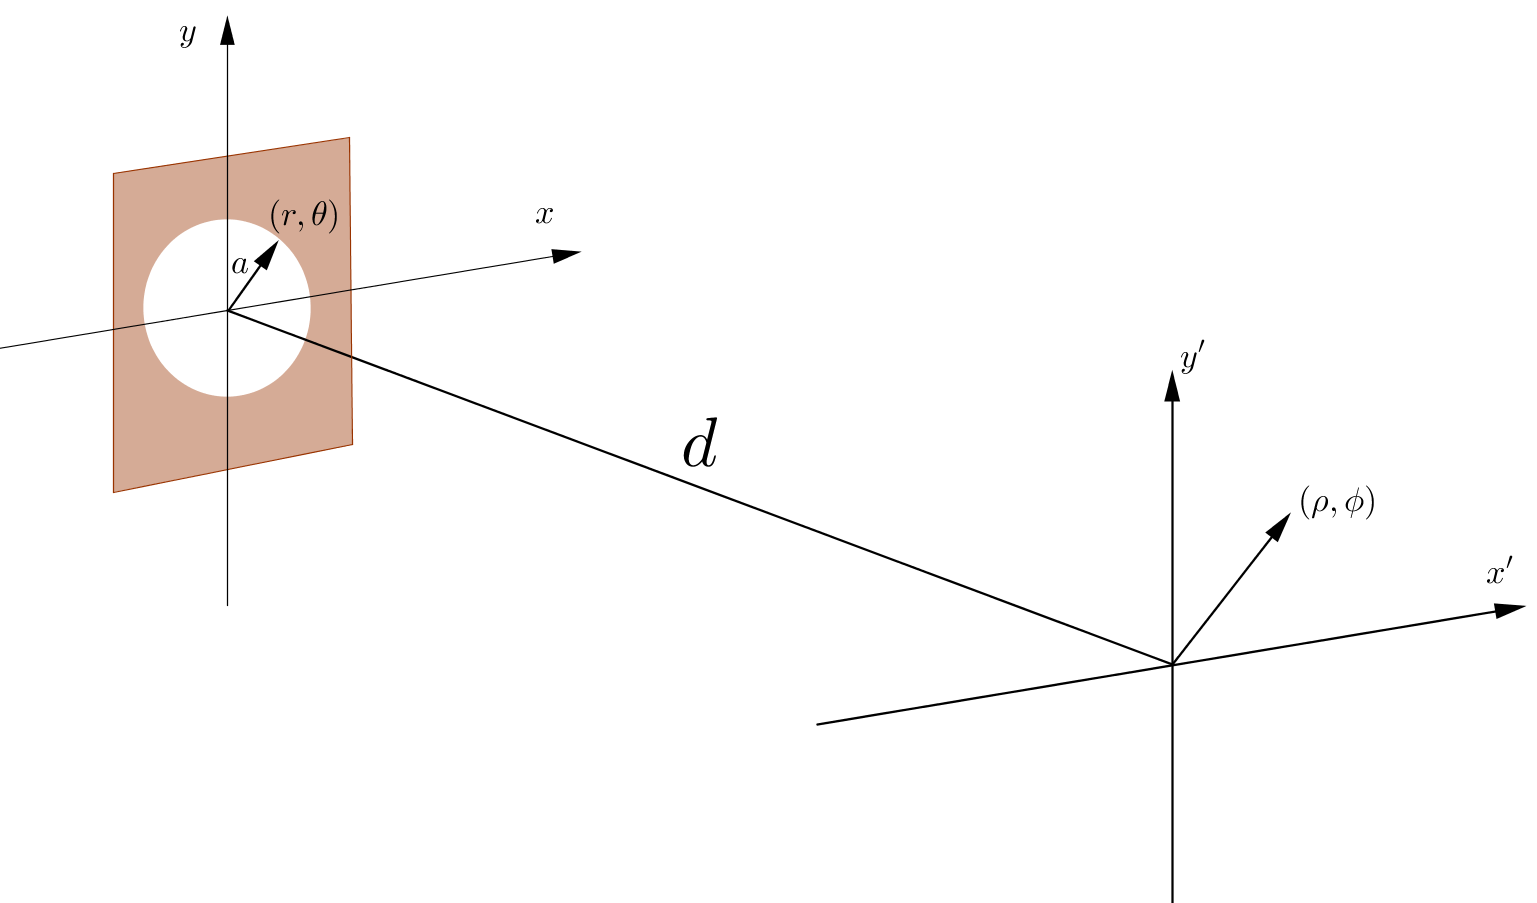
\includegraphics[width=0.75\linewidth]{Kap1/apertura_circ.png}
    \caption{Esquema  apertura circular aproximación de Fraunhofer.} 
    \label{esq_circular}
    \end{figure}
    
    En la figura \ref{esq_circular} se observa la simetría del problema en cuestión,como se ha visto la geometría de la abertura influye en el desarrollo de los cálculos por lo cual será más conveniente usar un sistema de coordenadas polar. Realizando un cambio de variables de la forma
    
    \begin{eqnarray}
        x&=&r\cos{\theta} \hspace{5mm} u=\rho \cos{\phi} \hspace{5mm} \rho = \sqrt{\frac{{x'}^2+{y'}^2}{\lambda ^2 d^2}}\\
        y&=&r\sin{\theta} \hspace{5mm} v=\rho \sin{\phi}.
    \end{eqnarray}
    Así pues,
    \begin{eqnarray}
        E(x',y')&=&\iint_{-\infty}^{\infty} E_0 circ\left( \frac{(x^2+y^2)^{1/2}}{a} \right) e^{-2\pi i(ux+vy)} dx dy\\
        E(\rho,\phi)&=& \int_{0}^{a} \int_{0}^{2\pi} E_0 e^{-2\pi i(\rho r \cos{\phi}\cos{\theta}+\rho r \sin{\phi}\sin{\theta})}rdrd\theta \\
        E(\rho,\phi)&=&E_0\int_{0}^{a} \int_{0}^{2\pi}e^{-2\pi i\rho r \cos{(\phi - \theta)}}rdrd\theta.
    \end{eqnarray}
    
    Usando la expresión de la función de Bessel de orden cero
    
    \begin{equation}
        J_0(u)=\frac{1}{2\pi}\int_{0}^{2\pi}e^{i u \cos{v}}dv,
    \end{equation}
    
    entonces la expresión para el campo queda
    
    \begin{equation}\label{campo_polares}
        E(\rho,\phi) = E_0 \frac{2\pi}{\lambda d} \int_{0}^{a} J_0(2\pi \rho r)rdr.
    \end{equation}
    Ahora usando la relación de recurrencia para las funciones de Bessel
    
    \begin{equation}\label{recurrencia_bessel}
        \frac{d}{du}\left[u^m J_m(u)\right]=u^m J_{m-1}(u) \hspace{4mm}\text{ para m=1  }\hspace{3mm} \frac{d}{du}\left[u J_1(u)\right]=u J_{0}(u),
    \end{equation}
    con lo cual usando (\ref{recurrencia_bessel}) en la ecuación (\ref{campo_polares}) solo queda evaluar la integral entre $0$ y $a$ quedando
    
    \begin{eqnarray}
        E(\rho,\phi)&=& E_0\frac{2\pi}{\lambda d} a^2 J_1(2\pi \rho a)\frac{1}{2\pi \rho a}\\
        E(\rho)&=& \left[ \frac{\pi a^2 E_0}{\lambda d}\right]\frac{2J_1(2\pi \rho a)}{2\pi \rho a},
    \end{eqnarray}
    con lo cual finalmente hallando el modulo al cuadrado para hallar la irradiancia tenemos
    
    \begin{equation}\label{irrad_circ}
        I(\rho)=I_0\left[\frac{2J_1(2\pi \rho a)}{2\pi \rho a}\right]^2  \hspace{3mm} \xrightarrow{\;\; \rho=r/\lambda d \;\; } \hspace{3mm}  I(r)=I_0\left[\frac{2J_1(\pi ar/\lambda d)}{(\pi ar/\lambda d)}\right]^2,
    \end{equation}
    la ecuación (\ref{irrad_circ}) nos muestra la irradiancia donde se observa una simetría en $\phi$ , es decir, el patrón generado serán anillos concéntricos. De ésta misma ecuación al igualar el primer cero de $J_1$ con su argumento, nos encontramos con la relación $r_a=1.22 \lambda d /a$, donde $r_a$ es llamado el \textbf{radio de Airy} y es precisamente la primera región de difracción para la abertura circular.\\
    De lo anterior nace el criterio de Rayleigt en el cual se indica que dos fuentes puntuales son resueltas por un observador si los centros de sus anillos de Airy están separados una distancia mayor a $r_a$.
\end{itemize}


\subsection{Rejilla de difracción.}
Las rejillas de difracción son un elemento óptico clave en cualquier instrumento de espectrometría, ya que con ella podemos descomponer la luz incidente en todas sus longitudes de onda constituyentes. Existen diversos tipos de rejillas con diferentes geometrías y materiales con lo cuales se obtiene una optimización en un rango del espectro electromagnético de interés. A continuación observaremos cuál es el principio teórico de manera muy similar a las aberturas circular y rectangular.\\

\begin{figure}[H]
    \centering
    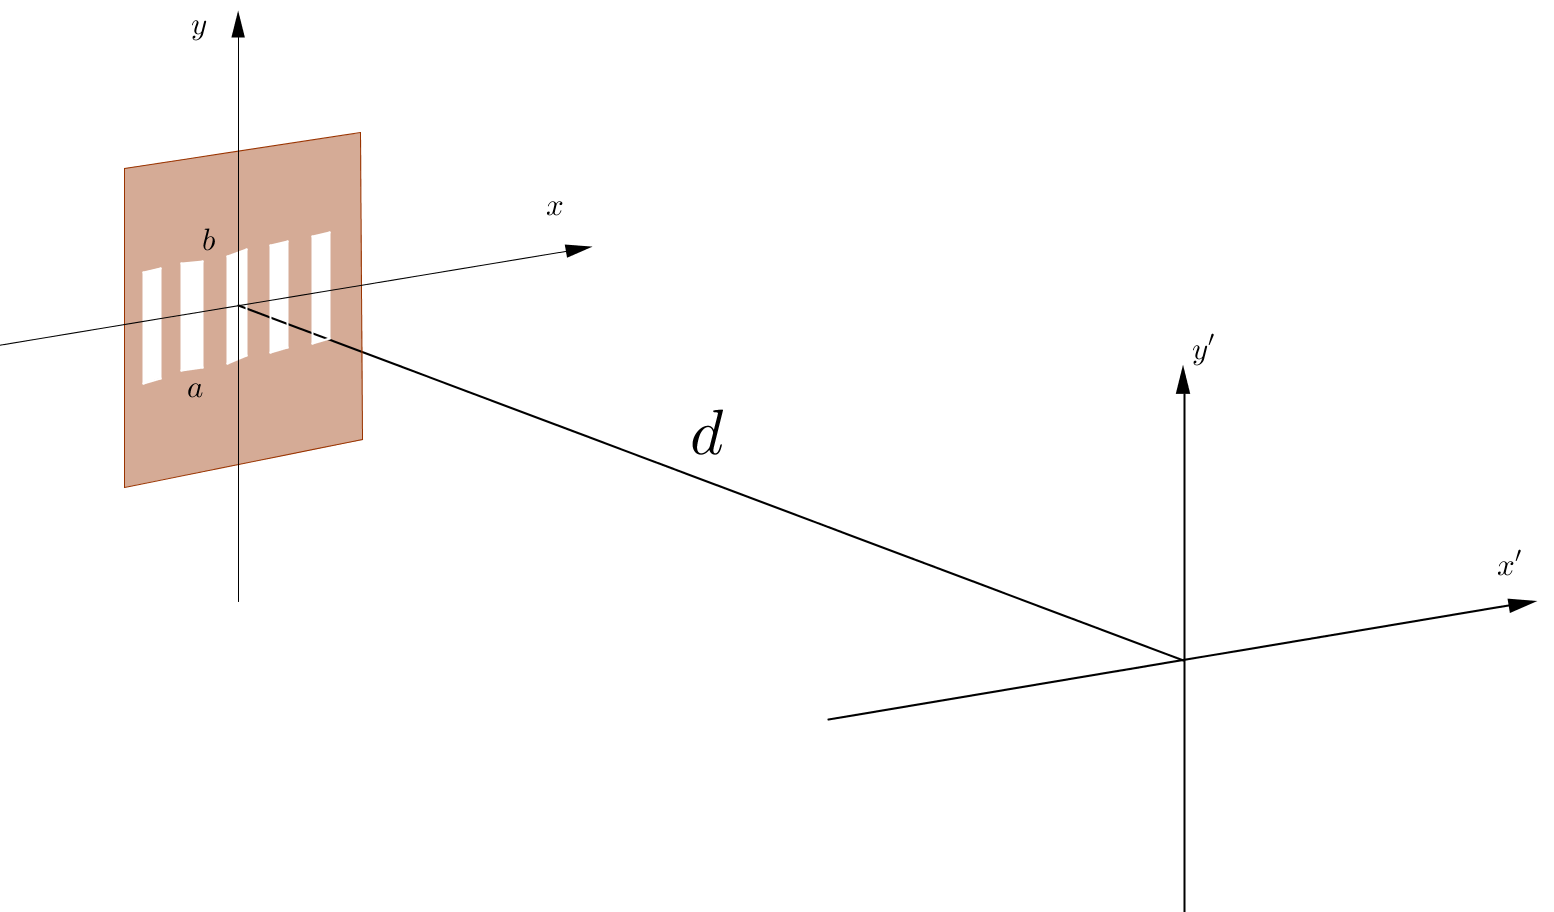
\includegraphics[width=0.8\linewidth]{Kap1/apertura_rejilla.png}
    \caption{Esquema para la rendija múltiple.} 
    \label{esq_rejilla}
\end{figure}
Como se observa en la figura \ref{esq_rejilla}, la rejilla se compone de $N$ rendijas rectangulares de ancho $a$ separadas una distancia $b$; con esta idea y usando la aproximación de Fraunhofer podemos superponer la solución ya encontrada para la apertura rectangular, con lo cual definimos la función rectángulo de la siguiente manera

\begin{equation}
    rect\left(\frac{x}{x_0}\right)=\left\lbrace
    \begin{array}{ll}
        \textup{si } |x|\leq {x_0}/2 & 1\\
        \textup{si } |x| \textup{ en otro caso.}
    \end{array}
    \right.
\end{equation}
Puesto que las aberturas se encuentran organizadas a lo largo del eje $x$, calcularemos la irradiancia que se produce a lo largo de este eje; de esta forma el campo $E$ en la dirección $x$ será el producto de la función rectángulo para una abertura desplazada $N$ veces, es decir, la convolución 

\begin{equation}\label{campo_rejilla}
    E(x)=E_0 \hspace{1mm} rect\left(\frac{x}{a}\right) \ast \sum_{n=0}^{N-1}\delta(x-nb) ,
\end{equation}
donde $N$ es el número de aberturas, $a$ el ancho y $b$ la separación entre los centros de las mismas.\\
Ahora aplicando la transformada de Fourier al campo y usando las propiedades de la convolución tenemos

\begin{eqnarray}\label{transf_rejilla}
    \mathcal{F}\lbrace E(x)\rbrace&=&\mathcal{F}\left \{ rect\left(\frac{x}{a}\right)\right \}\mathcal{F}\left \{ \sum_{n=0}^{N-1}\delta(x-nb)\right \}\\
    &=& a\hspace{1mm}sinc(\pi x' a) \left[ \sum_{n=0}^{N-1} e^{-2\pi i nbx'} \right].
\end{eqnarray}

Ahora calculando la suma mediante la resta de series tenemos

\begin{equation}
    S=\sum_{n=0}^{N-1} e^{-2\pi i nbx'} \hspace{10mm}S e^{-2\pi i bx'} = \sum_{n=1}^{N} e^{-2\pi i nbx'},
\end{equation}

con lo cual restando las series se obtiene

\begin{eqnarray}
    S\left(1-e^{-2\pi i bx'}\right)&=&1-e^{-2\pi i Nbx'}\\
    S&=&\frac{1-e^{-2\pi i Nbx'}}{1-e^{-2\pi i bx'}}=\frac{e^{-\pi i Nbx'}\left(e^{\pi i Nbx'}-e^{-\pi i Nbx'}\right)}{e^{-\pi i bx'}\left(e^{\pi i bx'}-e^{-\pi i bx'}\right)}\\
    S&=&e^{-\pi i (N-1) bx'}\left[\frac{\sin{(\pi N bx')}}{\sin{(\pi  bx')}}\right],
\end{eqnarray}

asi retomando la ecuación (\ref{transf_rejilla}) y hallando el módulo al cuadrado obtenemos 

\begin{equation}\label{irrad_rejilla}
    I(x')=I_0\hspace{1mm}{sinc}^2(\pi x' a) e^{-2\pi (N-1) bx'}\left[ \frac{\sin{(\pi N bx')}}{\sin{(\pi  bx')}} \right]^2 \hspace{3mm}\text{con}\hspace{3mm}I_0=\frac{E_{0}^{2} a^2}{\lambda^2 d^2},
\end{equation}
si suponemos muchas aberturas, $N\rightarrow\infty$
\begin{equation}\label{irrad_rejilla_Ngrande}
    I(x')=I_0\hspace{1mm}{sinc}^2(\pi x' a) \left[ \frac{\sin{(\pi N bx')}}{\sin{(\pi  bx')}} \right]^2,
\end{equation}
finalmete la ecuación (\ref{irrad_rejilla_Ngrande}) nos describe el patrón de difracción para la rejilla constituida por múltiples aberturas, esta ecuación nos muestra por un lado el valor máximo $I_0$ que puede tomar la función, otro término que expresa la irradiancia generada a partir de una única abertura y un término final correspondiente a la interferencia generada por las $N$ aberturas.
%%%%%----------------------------------------------%%%%%
%%%%----------------------------------------------%%%%

\subsection{Integrated Fiber Unit (IFU).}

En la actualidad existen dispositivos tanto de imagen como espectrógrafos que utilizan múltiples fibras ópticas en el diseño de los mismos. A los instrumentos que usan este enjambre de fibras ópticas se les conoce como IFU, acrónimo en inglés correspondiente a \textit{Integrated Fiber Units}. Un ejemplo de estos es el instrumentos SINFONI \textit{Spectrometer for Infrared Faint Field Imaging}.\\
Además de SINFONI se encuentran en desarrollo e incluso construcción diversos instrumentos los cuales desean obtener información espectroscópica de algún objeto astronómico en un mismo instante de tiempo, en éste caso el objeto de interés es el Sol el cual nos lleva a superar diversos retos puesto que es una fuente de gran intensidad. Superando éstos desafíos a la hora de obtener información del Sol se expondrán 3 proyectos IFU's con cualidades ópticas diferentes \textbf{multi Slit}, \textbf{multi fibra} y \textbf{multi lentes}, los cuales proponen construir imágenes del Sol con gran resolución espacial y espectral en un amplio rango de longitudes de onda (hacia el IR cercano), éstos instrumentos están diseñados para telescopios terrestres.\\

El primer instrumento \textbf{multi Slit} llamado \textbf{MuSICa} \textit{Multi Slit Image Slicer on collimator Camera} del IAC, diseñado para el telescopio terrestre Gregor de 1,5m se compone de una mascara dividida en 2 segmentos, con lo cual cada segmento de la imagen es dirigido con ayuda de espejos a una mascara con 4 slits, nuevamente cada slit es redirigido con ayuda de espejos a una disposición vertical donde finalmente la luz es dispersada por una rejilla de reflexión cóncava esférica y registrada con un detector igualmente cóncavo esférico. Así se obtiene una imagen compuesta por 8 slits con un ancho de 100 $\mu$m y altura 1,8 mm, el hecho de que la luz no atraviesa ningún elemento óptico disminuye los efectos de aberración generando una mayor calidad de la imagen espectroscópica.\\ 

El segundo instrumento \textbf{multi fibra} es diseñado para el telescopio de 4m DKIST, en este caso se cuentan con diversos proyectos con longitudes de onda en el rango visble e IR cercano y lejano. Pero en especial hablaremos del \textbf{DL-NIRSP} "Diffraction-Limited-Near-Infrared SP" del NSO.

\begin{figure}[H]
\centering
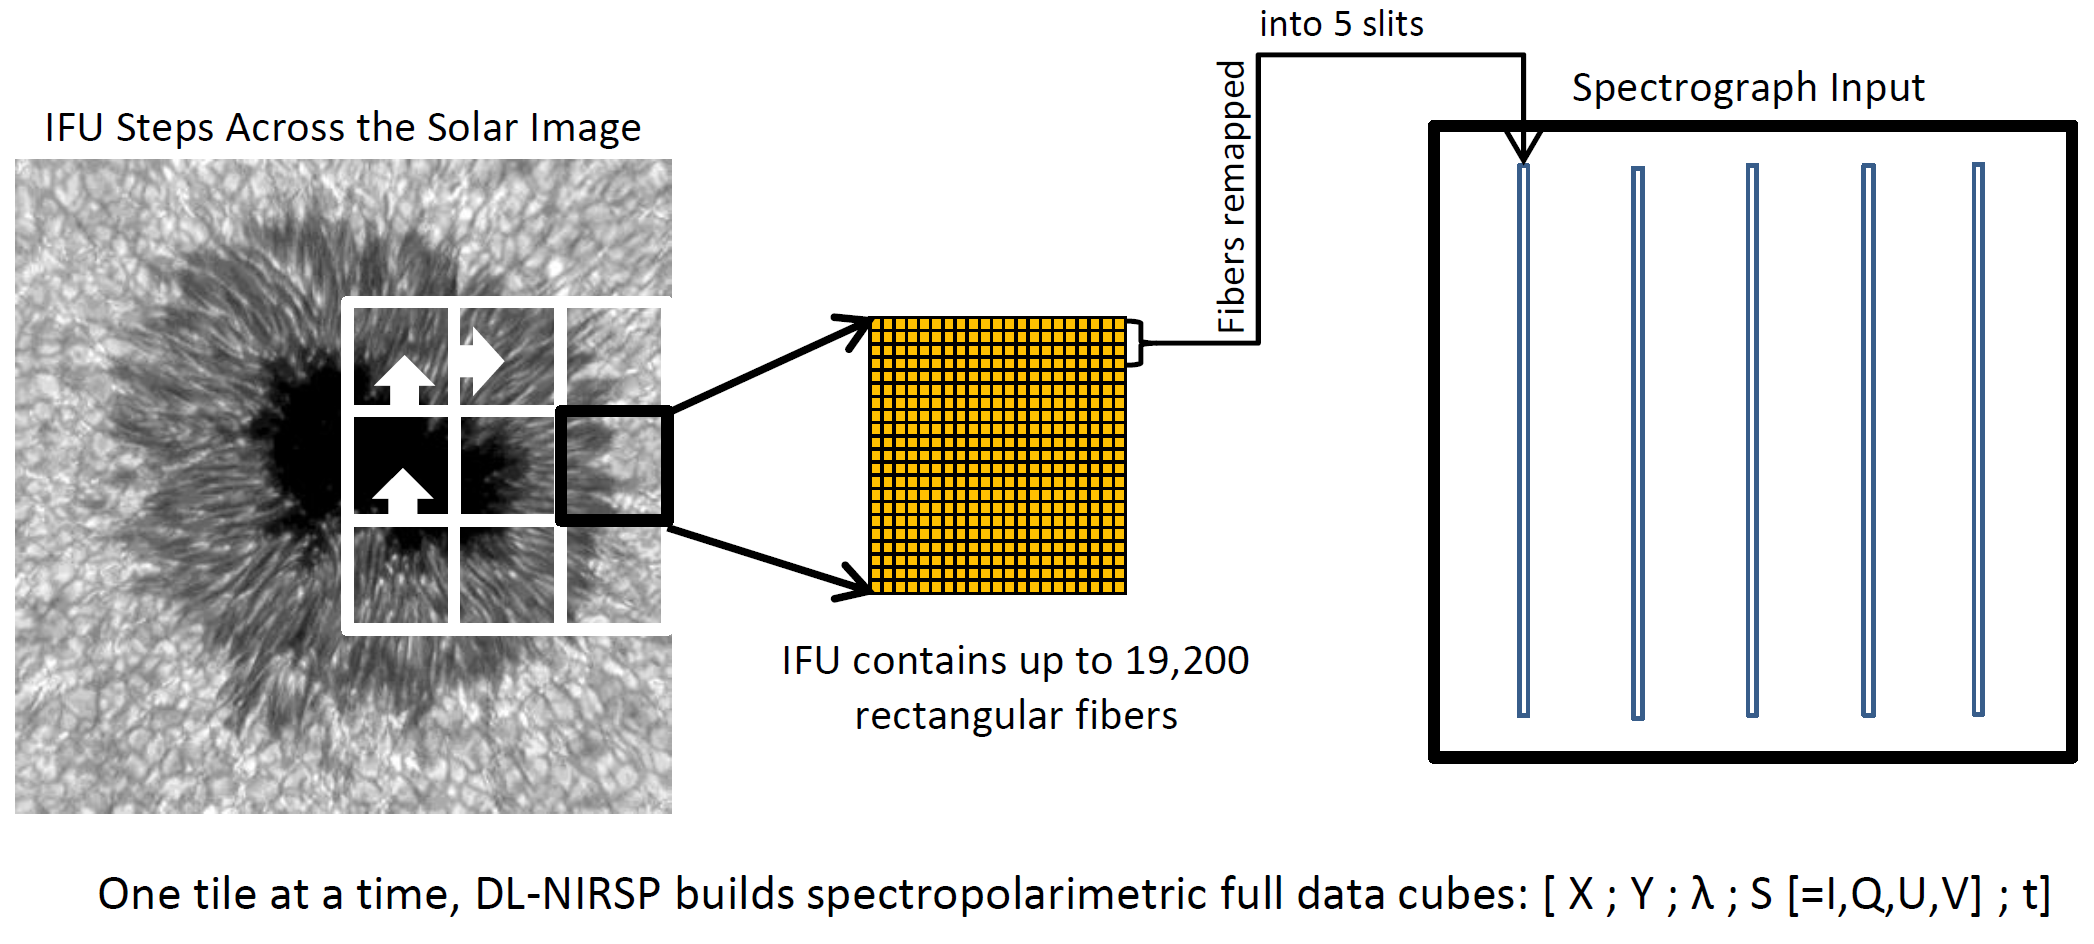
\includegraphics[width=0.70\linewidth]{Kap1/nirsp.png}
\caption{Esquema del funcionamiento para el instrumento DL-NIRSP del NSO. Tomado de \textit{https://www.nso.edu/telescopes/dkist/instruments/dl-nirsp}} 
\label{nirsp}
\end{figure}

Como se observa en la figura \ref{nirsp} el instrumento cuenta con un arreglo de fibras cuadradas (19200) con las cuales se mapea la región del Sol en interés (9 zonas), después las fibras son organizadas en un arreglo lineal de 5 Slit donde posteriormente se descompone la luz con ayuda de una rejilla de reflexión cóncava que finalmente será registrada por el detector. Dicha disposición logra que el instrumento tenga un campo de visión de 120x120 arcsec y una resolución espectral $R\aprox250000$ analizando estados Full de polarización de las lineas espectrales en la rango 900-2500 nm con una cadencia temporal menor a 100 ms, dado éste rango de operación el instrumento estudia la cromosfera Solar en regiones activas donde pueden producirse Flares.\\

Por último el instrumento \textbf{multi lentes} denominado \textbf{Mihi} del MPS el cual se compone de un arreglo de fibras ópticas que a su vez cuentan con microlentes los cuales reducen el tamaño del píxel al capturar mayor información en el plano imagen del telescopio.

\begin{figure}[H]
\centering
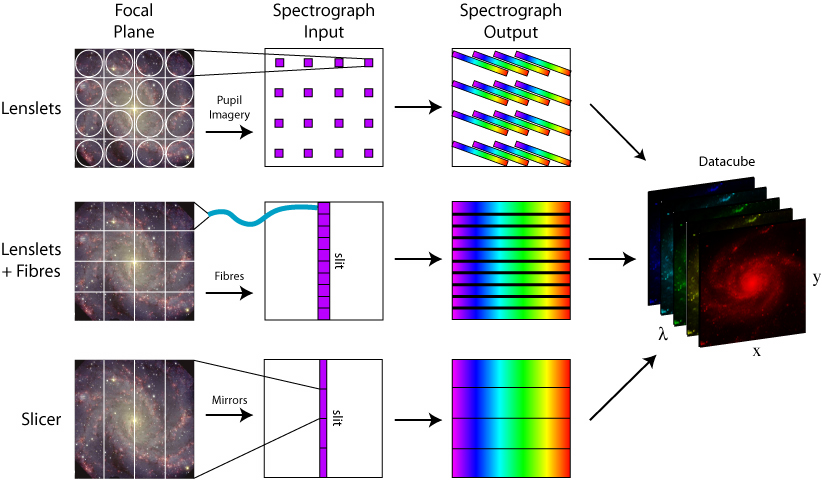
\includegraphics[width=0.70\linewidth]{Kap1/multilentes.jpg}
\caption{Diferencias en el diseño para la obtención de datos en los diferentes IFU's. M. Westmoquette, adapted from Allington-Smith et al. 1998 ,Recuperado de \textit{http://ifs.wikidot.com}.} 
\label{multilente}
\end{figure}

El funcionamiento en éste caso es muy similar al DL-NIRSP como se muestra en la figura \ref{multilente}, con la diferencia que se añaden microlentes para capturar más información, el transporte de la información también se da por fibra óptica al igual que el uso de una rejilla de reflexión y detector cóncavos. Al introducir microlentes se añade una dispersión espectral como se ejemplifica en la figura \ref{multilente} lo cual hace que se tengan que usar nuevos algoritmos para la obtención final de datos.




